%This is a LaTeX template for homework assignments
\documentclass{article}
\usepackage[utf8]{inputenc}
\usepackage{amsmath}
\usepackage{float}
\usepackage{placeins}
\usepackage{graphicx}
\usepackage{multicol}
\usepackage[spanish,es-nodecimaldot]{babel}
\usepackage{parskip}
\usepackage{geometry}
\usepackage{amssymb}
 \geometry{
 %total={170mm,257mm},
 top=20mm,
 bottom=20mm,
 left=20mm,
 right=20mm
 }


\begin{document}

\section*{Tarea 2}

Nombres: Mario Becerra, Miguel Vilchis \\
Fecha: Agosto 2016

%%%%%%%%%%%%%%%%%%%%%%%%%%%%%%%%%%%%%%%%
%%% Pregunta 1
%%%%%%%%%%%%%%%%%%%%%%%%%%%%%%%%%%%%%%%%

\subsection*{1.- Demostrar que las siguientes funciones son $\Theta(n^2)$ Mostrar $n_0$, $c_1$ y $c_2$.}
\textit{Nota:} Se dice que una función  $f \in \Theta(g(n))$ si existen $c_1, c_2 \in \mathbb{R}$, con $c_1, c_2 > 0$ y $n_0 \in \mathbb{N}$ tal que $\forall n \geq n_0$ se cumple que
\[ c_2 g(n) \leq f(n) \leq c_1 g(n) \].

\begin{enumerate}

    %%%%%%%%%%%%%%%%
    %%% 1
    %%%%%%%%%%%%%%%%
    \item $60n^2 + 5n +1$ \\
    \begin{multicols}{2}
    \begin{center}(1) \end{center}
    La desigualdad: $c_2  n^2 \leq 60n^2 + 5n +1 $ \\
         se cumple si y solo si: \\
         $c_2 \leq 60 + \frac{5}{n} + \frac{1}{n^2}$ 
    \columnbreak
     \begin{center}(2) \end{center}
    La desigualdad: $c_1  n^2 \geq 60n^2 + 5n +1 $ \\
         se cumple si y solo si: \\
         $c_1 \geq 60 + \frac{5}{n} + \frac{1}{n^2}$ 
    \end{multicols}
    De (1) es fácil ver que $\forall n \geq 1$ se tiene que $ 60 + \frac{5}{n} + \frac{1}{n^2} \leq 50+5+1 = 66$. Y de (2) tenemos que $\forall n \geq 1$ se cumple con $60 + \frac{5}{n} + \frac{1}{n^2} \geq 60$. De aquí tomando a $n_0 =1$, $c_2= 66$ y $c_1 = 60$ se cumple :
    \[\forall n \geq n_0 \rightarrow 60n^2 \leq 60n^2 + 5n +1 \leq 66n^2 \]
    $\therefore 60n^2 + 5n +1 \in \Theta(n^2)$
    
    %%%%%%%%%%%%%%%%
    %%% 2
    %%%%%%%%%%%%%%%%
    
    \item $2n^2 -16n +35$
    
    \begin{multicols}{2}
    \begin{center}(3) \end{center}
     La desigualdad: $c_2  n^2 \leq  2n^2 -16n +35$ \\
         se cumple si y solo si: \\
         $c_2 \leq 2 - \frac{16}{n} + \frac{35}{n^2}$ 
    \columnbreak
     \begin{center}(4) \end{center}
    La desigualdad: $c_1  n^2 \geq  2n^2 -16n +35$ \\
         se cumple si y solo si: \\
         $c_1 \geq 2 - \frac{16}{n} + \frac{35}{n^2}$ 
    \end{multicols}
    Por (3) tenemos que  $\forall n \geq 4$ se tiene que $\frac{16}{n} \geq \frac{35}{n^2}$ por lo que $2 \geq 2 -(\frac{16}{n} - \frac{35}{n^2})$ .
    Por otro lado por la desigualdad (4) para valores de $n \geq 16$ se tiene que $2 - \frac{16}{n} + \frac{35}{n^2} \geq 2-1+\frac{35}{n^2} \geq 1$.
    De esto, tomamos $n_0 = 16$, $c_1 = 2$ y $c_2 = 1$  se cumple :
    \[\forall n \geq 16 \rightarrow n^2 \leq 2n^2 -16n +35 \leq 2  n^2 \]
    $\therefore2n^2 -16n +35\in \Theta(n^2)$
    
    %%%%%%%%%%%%%%%%
    %%% 3
    %%%%%%%%%%%%%%%%
    
    \item $3n^2 + 2  n log(n) $\\
    
    \textit{Nota: } La función $f(n) = n -log(n)$ es creciente para $n \geq 1$, y además $\forall  n \geq 1$ se cunmple que $n\geq log(n)$.
    \begin{multicols}{2}
    \begin{center}(5) \end{center}
    Evidentemente se cumple:  \\
     $3n^2 + 2  n log(n) \geq 3n^2$
    \columnbreak
     \begin{center}(6) \end{center}
    Por la nota tenemos que:\\
    $3n^2 + 2  n log(n) \leq  3n^2 + 2  n  n$\\
    $ 3n^2 + 2  n  n =  5n^2$
    \end{multicols}
    
    
    Como las desigualdades se cumplen $\forall n \geq 1$ y por lo ya mencionado, si tomamos $n_0 = 1$, $c_1 = 5$ y $c_2 = 3$ se cumple: 
    
    \[\forall n \geq 1 \qquad 3  n^2 \leq 3n^2 + 2  n log(n)  \leq 5  n^2 \]
    $\therefore 3n^2 + 2  n log(n) \in \Theta(n^2)$
    
    %%%%%%%%%%%%%%%%
    %%% 4
    %%%%%%%%%%%%%%%%
    
    \item $2+4+6+... +2n$ \\
    \textit{Nota:} La expresión $2+4+6+...+2  n$ es equivalente a:
    \[\sum_{i=1}^n 2 i = 2 \sum_{i=1}^n i \]
    \[ 2 \sum_{i=1}^n i = n *(n-1)\]
    
    \begin{multicols}{2}
    \begin{center}(7) \end{center}
     La desigualdad: $c_2  n^2 \leq  n^2-n$ \\
         se cumple si y solo si: \\
         $c_2 \leq 1 - \frac{1}{n}$ 
    \columnbreak
     \begin{center}(8) \end{center}
    La desigualdad: $c_2  n^2 \geq  n^2-n$ \\
         se cumple si y solo si: \\
         $c_2 \geq 1 - \frac{1}{n}$
    \end{multicols}
    Si tomamos $n_0 = 2$, $c_1 =1$, y $c_2 = \frac{1}{2}$, con lo que se cumple que : 
    \[\forall n \geq 2 \rightarrow \frac{1}{2}  n^2 \leq n^2 -n  \leq n^2 \]
    $\therefore n^2 + n  \in \Theta(n^2)$
    
    %%%%%%%%%%%%%%%%
    %%% 5
    %%%%%%%%%%%%%%%%
    
    \item 
    \begin{verbatim}
for i = 1:n
    for j = 1:i
        for k = 1:j
            x = x + 1
    \end{verbatim}
    
    El costo del código de arriba es 
    \begin{equation}
    \label{ej_1_5}
    \sum_{i = 1}^n \sum_{j = 1}^i \sum_{k = 1}^i c    
    \end{equation}
    
    donde $c$ es un costo fijo por operación. Simplificando las sumas en la ecuación \ref{ej_1_5} se llega a que

    \begin{align}
        \sum_{i = 1}^n \sum_{j = 1}^i \sum_{k = 1}^i c &= 
        c \sum_{i = 1}^n \sum_{j = 1}^i j \\
        &=  c \sum_{i = 1}^n \frac{i(i + 1)}{2} \\
        &= \frac{c}{2} \left[ \sum_{i = 1}^n i^2 + \sum_{i = 1}^n i \right] \\
        &= \frac{c}{2} \left[ \frac{n(n + 1)(2n + 1)}{6} + \frac{n(n+1)}{2} \right] \\
        &= an^3 + bn^2 + dn
    \end{align}
    
    con $a = \frac{c}{6}, b = \frac{c}{2}, d = \frac{c}{3}$.
    
    %Para el código de arriba haremos un análisis de operaciones. La línea 1 toma $c_1  n$ operaciones, que son los incrementos de $i$ y la comparación booleana, para alguna constante $c_1$.
    %
    %En la línea 2, la cantidad de operaciones que se van a realizar son $\sum_{j=1}^i c_2 j$ para alguna constante $c_2$, note que es equivalente a $c_2 \sum_{j = 1}^i j = c_2 (\frac{(n+1) n}{2})$.
    %
    % Para la línea 3 y 4, lo que tenemos es $\sum_{k=1}^i c_3  k^2 = c_3  (\frac{(n (n+1)  (2n+1))}{6})$.
    
    Con lo que concluimos que la complejidad del código está dada por:
    \[ 
    p(n) = an^3 + bn^2 + dn.
    \]
    
    Lo que implica que el polinomio $p(n) \in \Theta(n^3)$. Se sabe que si una función $g \in \Theta(n^3)$ entonces $g \notin \Theta(n^2)$, por lo que $p(n) \notin \Theta(n^2)$.
    
\end{enumerate}


%%%%%%%%%%%%%%%%%%%%%%%%%%%%%%%%%%%%%%%%
%%% Pregunta 2
%%%%%%%%%%%%%%%%%%%%%%%%%%%%%%%%%%%%%%%%

\subsection*{2.- Ordenar las siguientes funciones de acuerdo a su tasa de crecimiento.}

\begin{figure}[H]
\centering
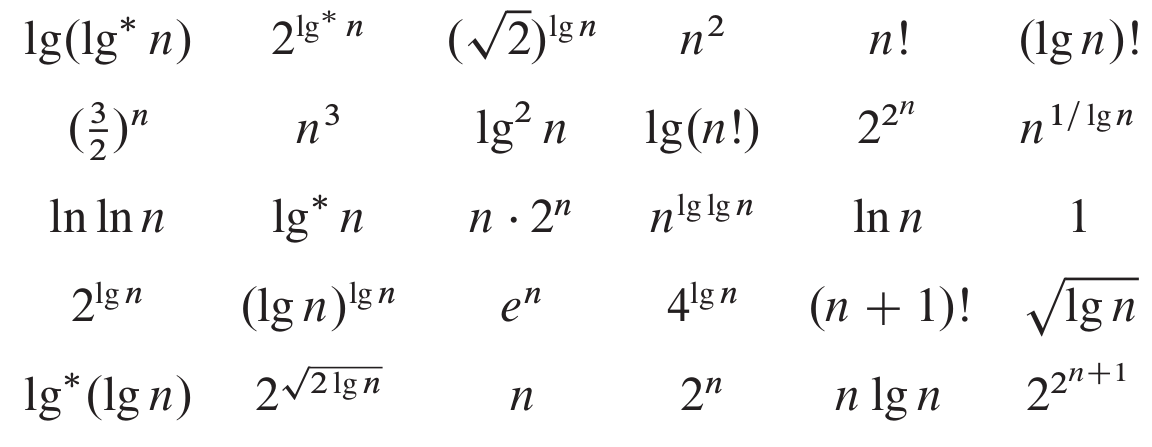
\includegraphics[width=0.5\textwidth]{img/ecuaciones_preg2.png}
\end{figure}

Esto se puede resolver de forma gráfica. El ordenamiento final es

\begin{enumerate}
\def\labelenumi{\arabic{enumi}.}
\itemsep1pt\parskip0pt\parsep0pt
\item
  $2^{2^{n+1}}$
\item
  $2^{2^{n}}$
\item
  $(n+1)!$
\item
  $n!$
\item $e^n$
\item $n 2^n$
\item $2^n$
\item $(\frac{3}{2})^n$
\item $\textrm{lg}(n)^{\textrm{lg}(n)} = n^{\textrm{lg}( \textrm{lg}(n))}$ 
\item $(\textrm{lg}(n))!$
\item $n^3$
\item $n^2 = 4^{\textrm{lg}(n)}$ 
\item $\textrm{lg}(n!)$
\item $n = 4^{\textrm{lg}(n)}$
\item $\sqrt{2}^{\textrm{lg}(n)}$
\item $2^{\sqrt{2 \textrm{lg}(n)}}$
\item $\textrm{lg}^2(n)$
\item $\ln (n)$
\item $\sqrt{\textrm{lg}(n)}$
\item $\ln(\ln(n))$
\item $2^{\textrm{lg}^*(n)}$
\item $\textrm{lg}^*(n)$
\item $\textrm{lg}^*(\textrm{lg}(n))$
\item $\textrm{lg}(\textrm{lg}^*(n))$
\item $n^{\frac{1}{\textrm{lg}(n)}}$
\item $1$
\end{enumerate}

Las gráficas de las funciones se pueden ver a continuación, donde 'ec\_n' se refiere a la ecuación n-ésima ecuación yendo de izquierda a derecha y de arriba a abajo.


\begin{figure}[H]
\centering
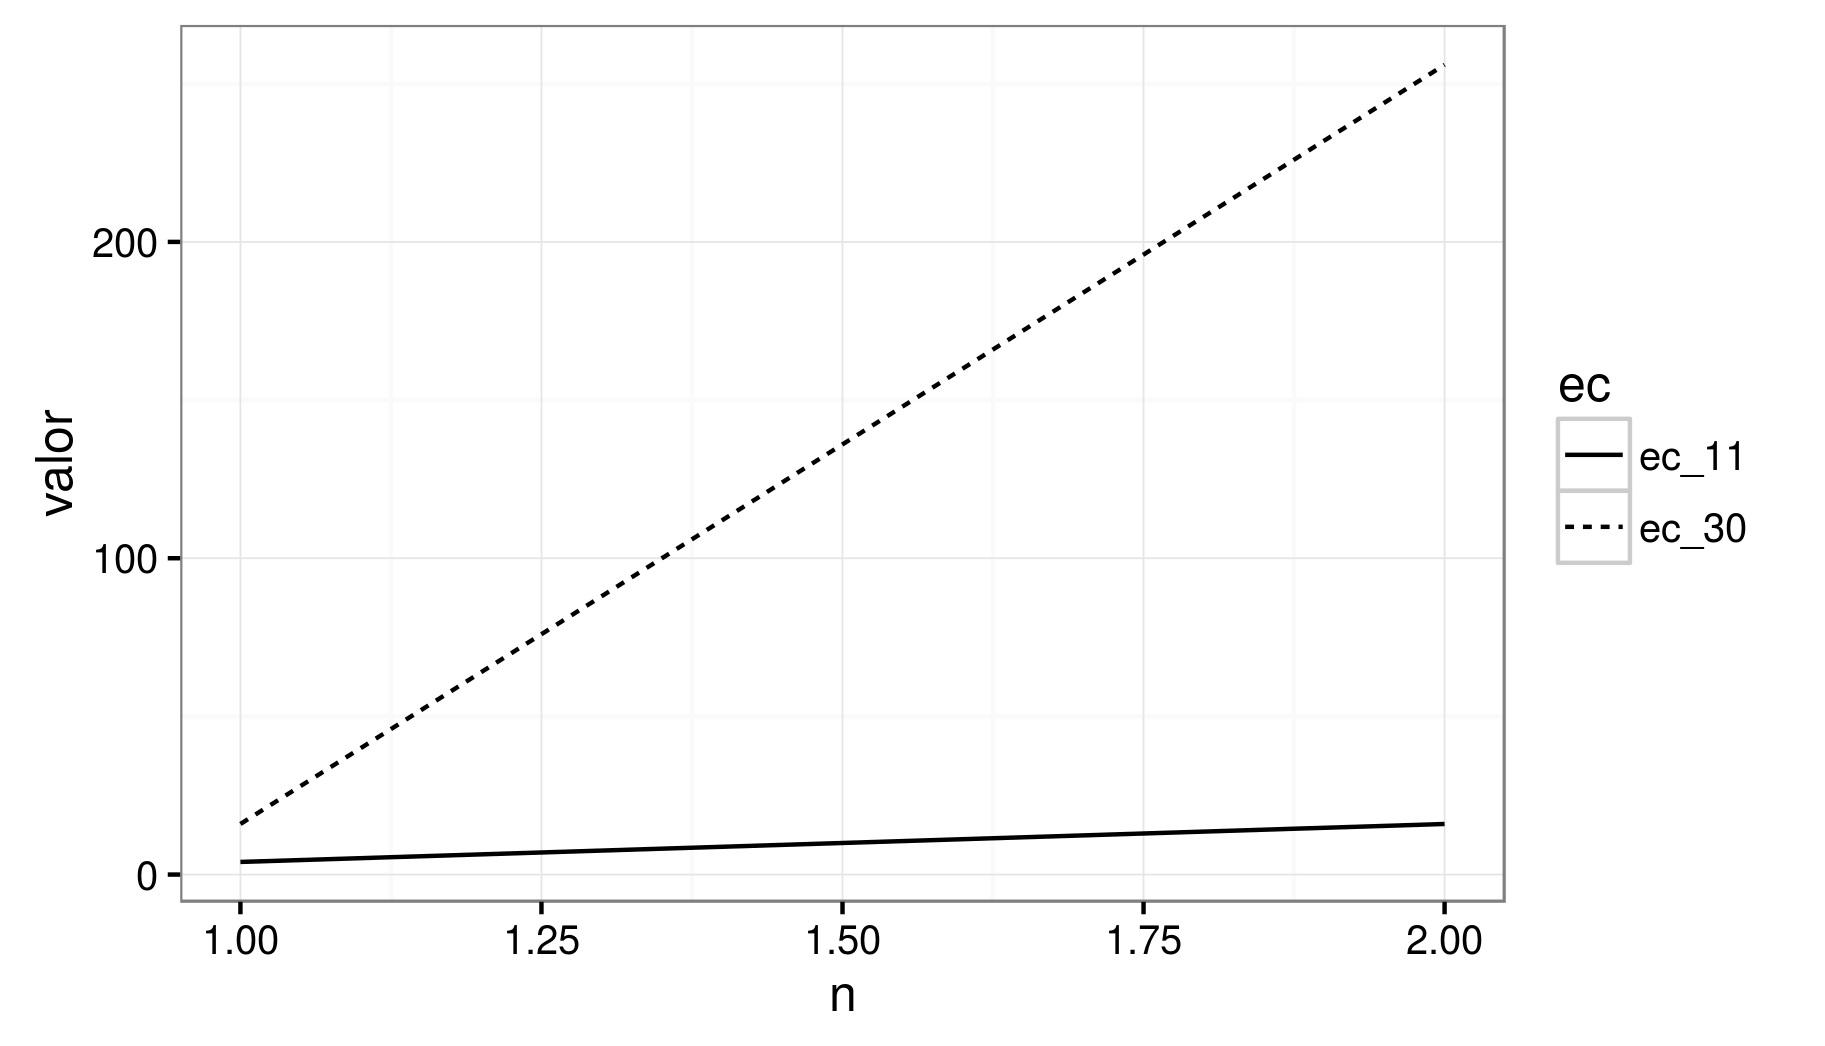
\includegraphics[width=0.5\textwidth]{img/graf_01.png}
\end{figure}

\begin{figure}[H]
\centering
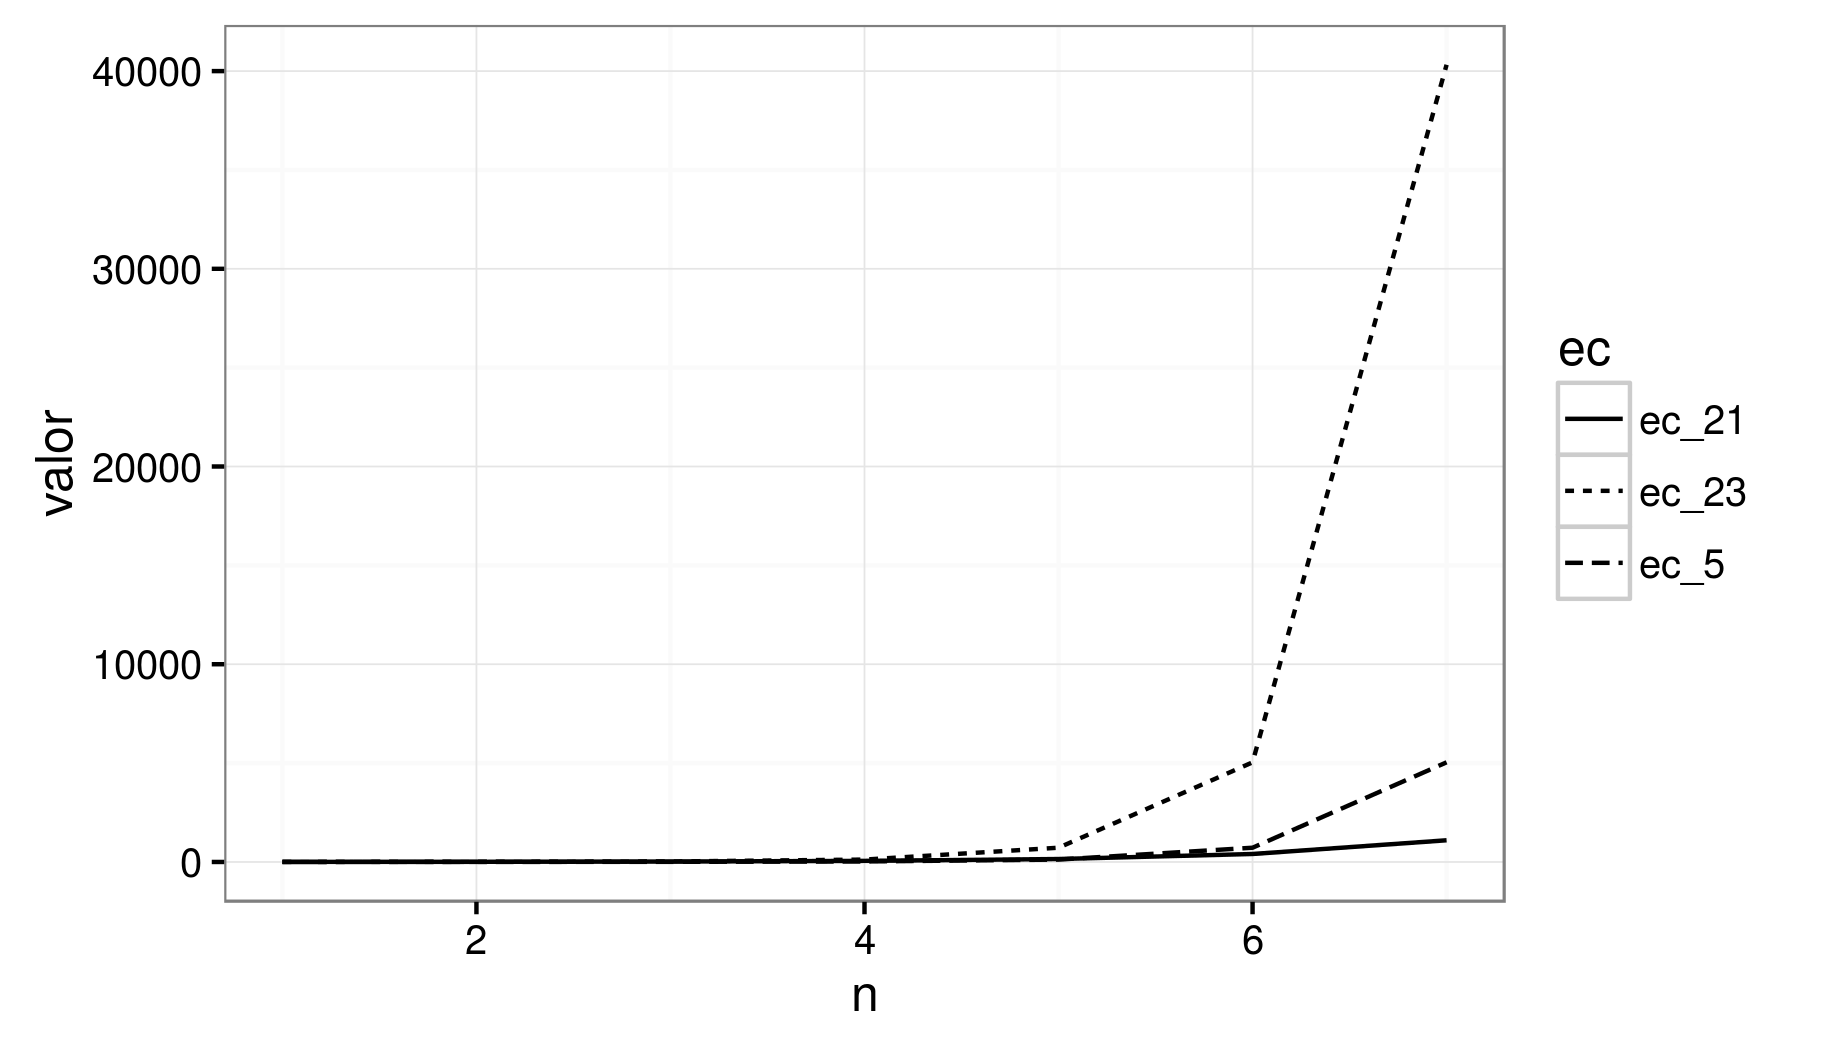
\includegraphics[width=0.5\textwidth]{img/graf_02.png}
\end{figure}

\begin{figure}[H]
\centering
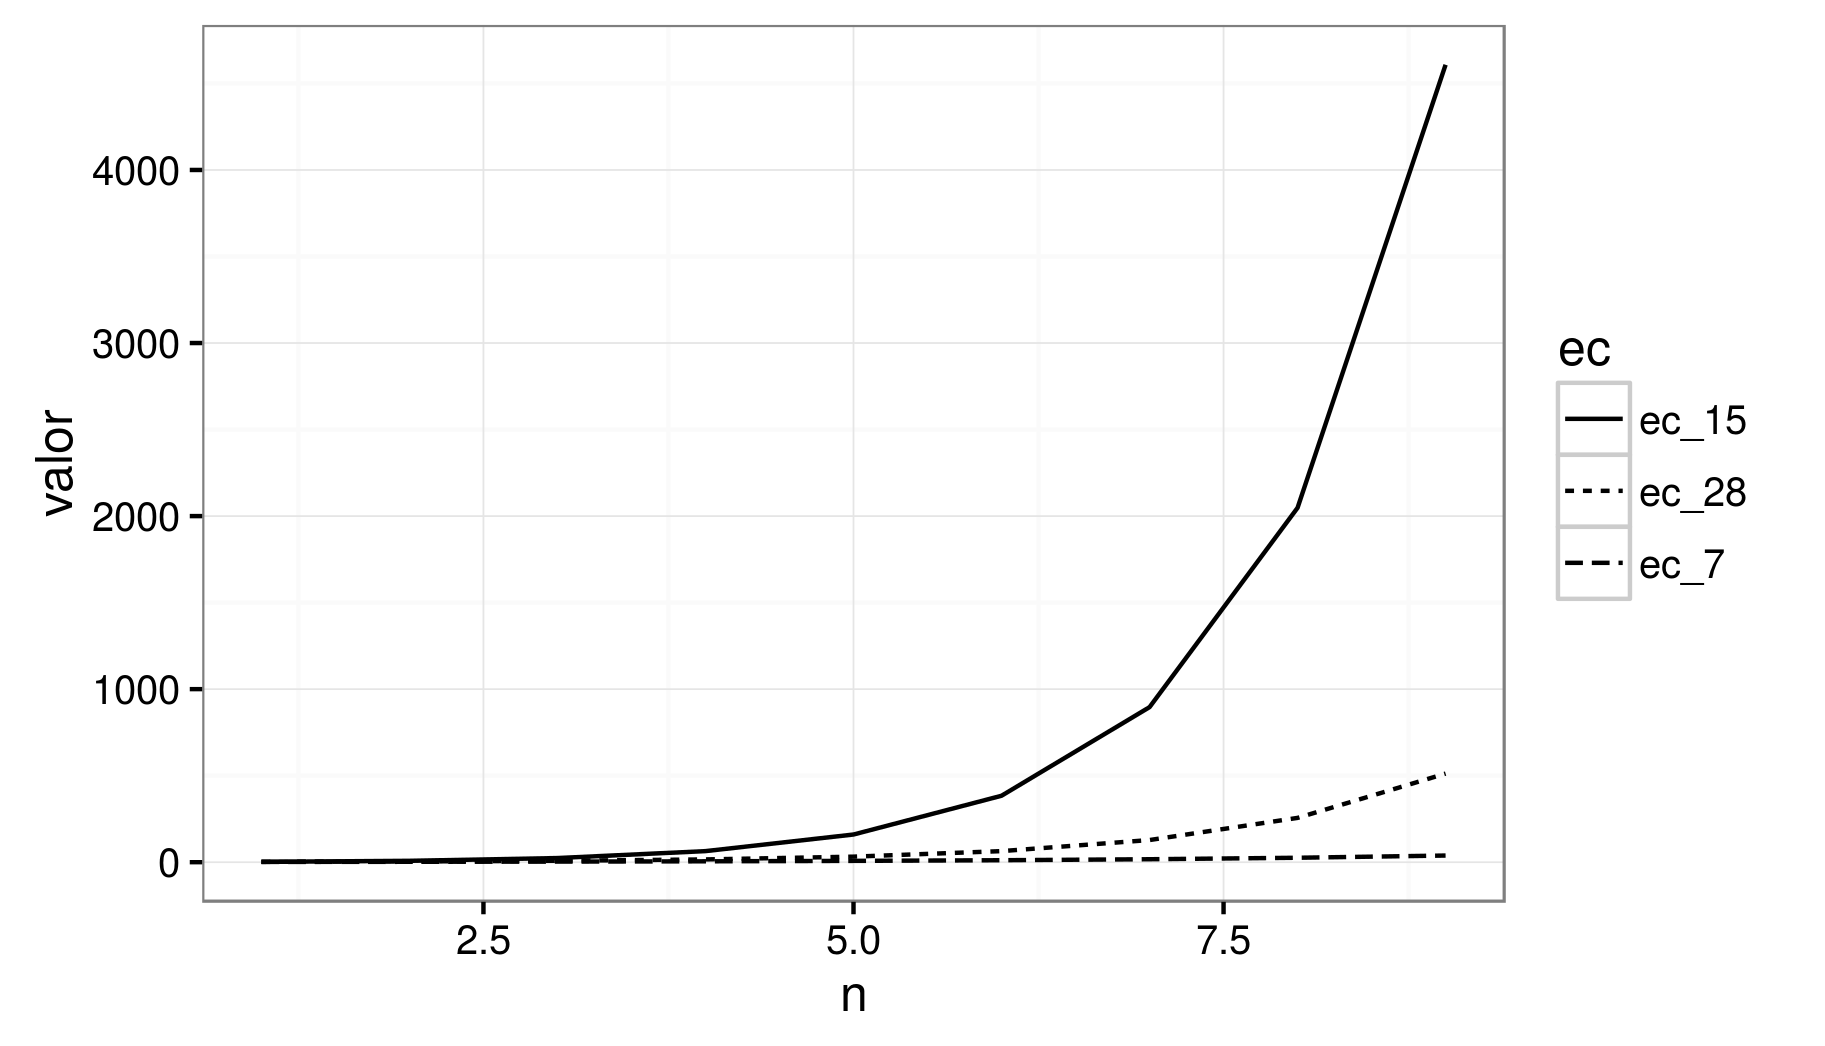
\includegraphics[width=0.5\textwidth]{img/graf_03.png}
\end{figure}

\begin{figure}[H]
\centering
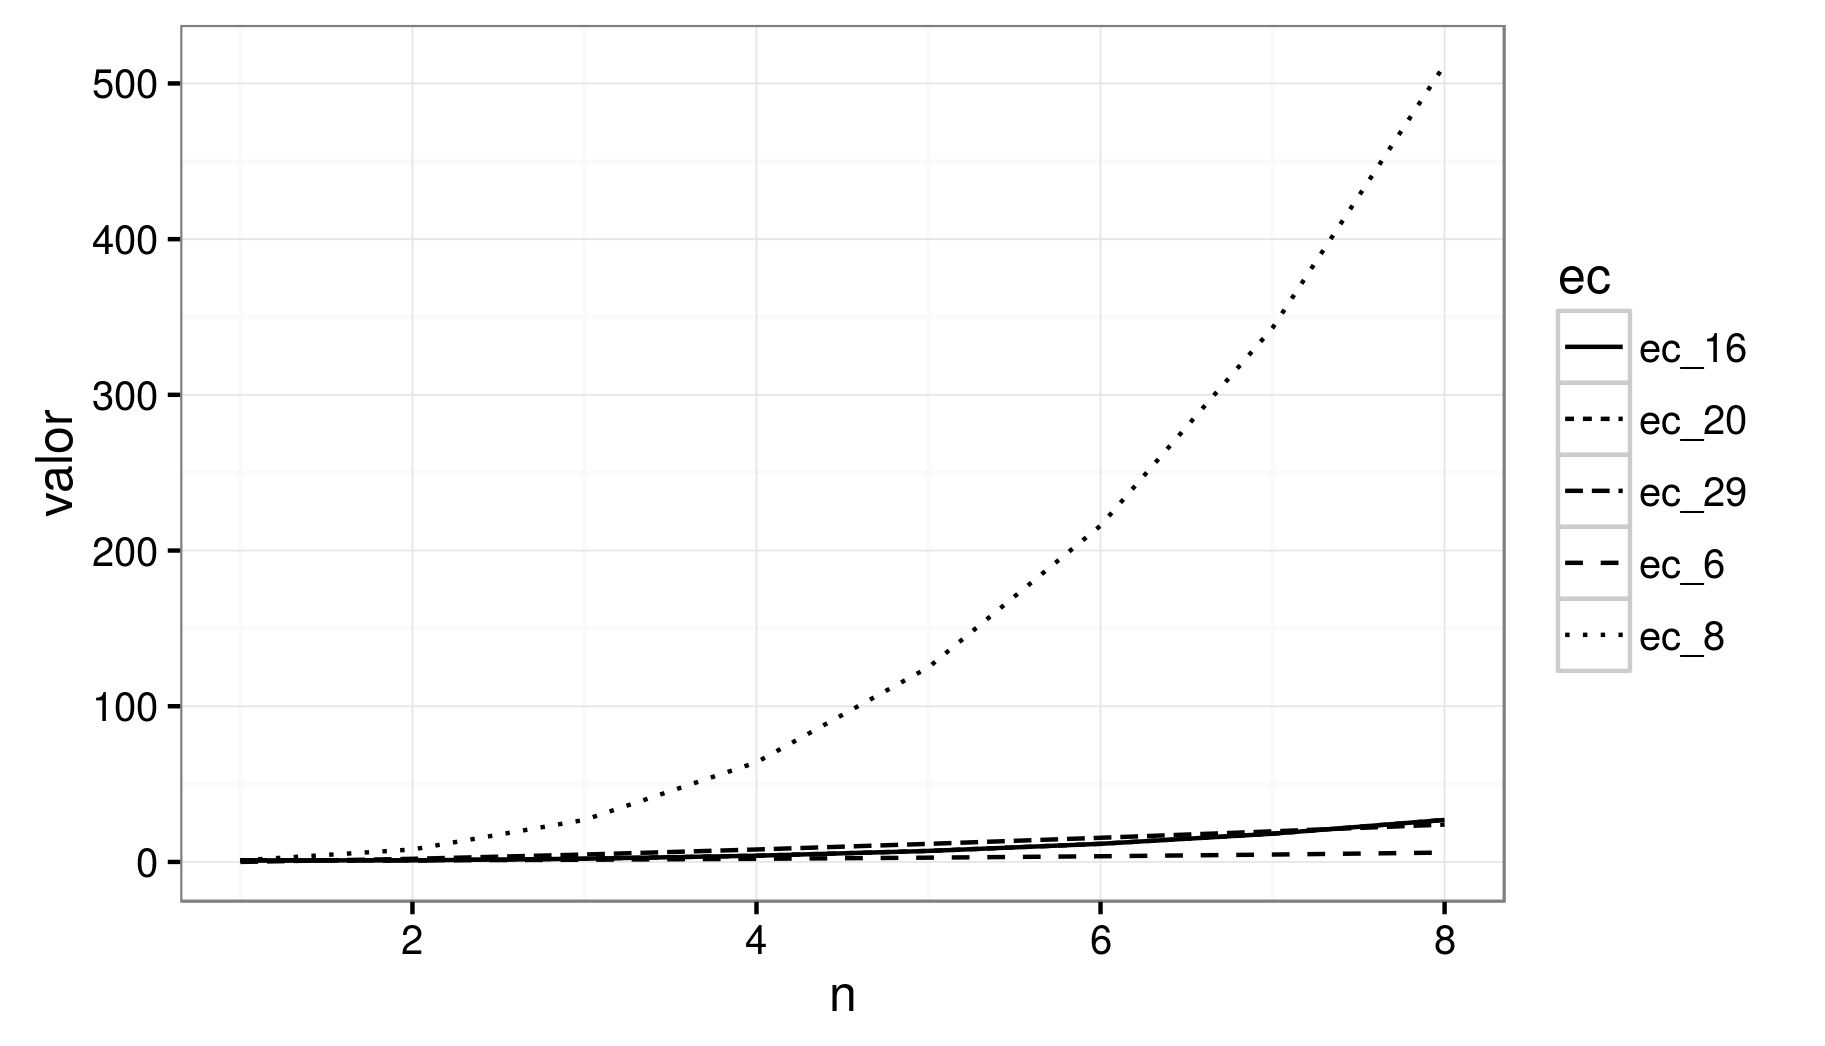
\includegraphics[width=0.5\textwidth]{img/graf_04.png}
\end{figure}

\begin{figure}[H]
\centering
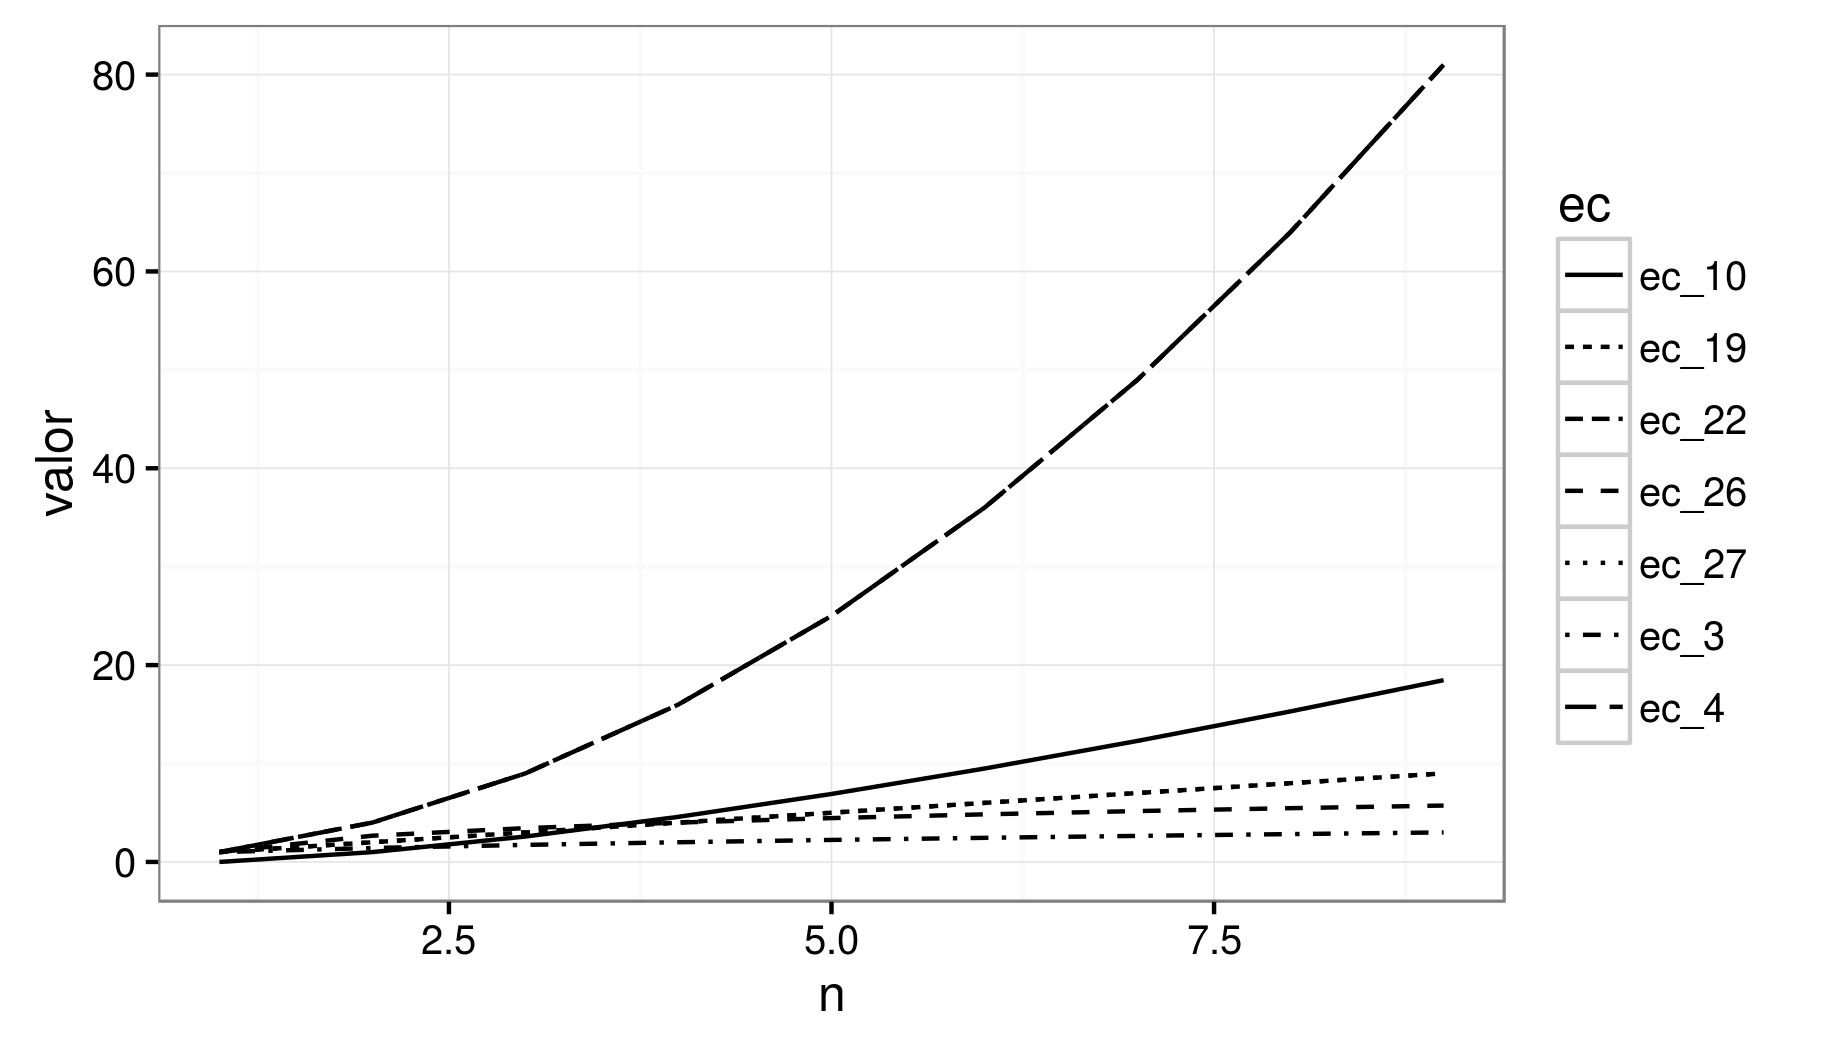
\includegraphics[width=0.5\textwidth]{img/graf_05.png}
\end{figure}

\begin{figure}[H]
\centering
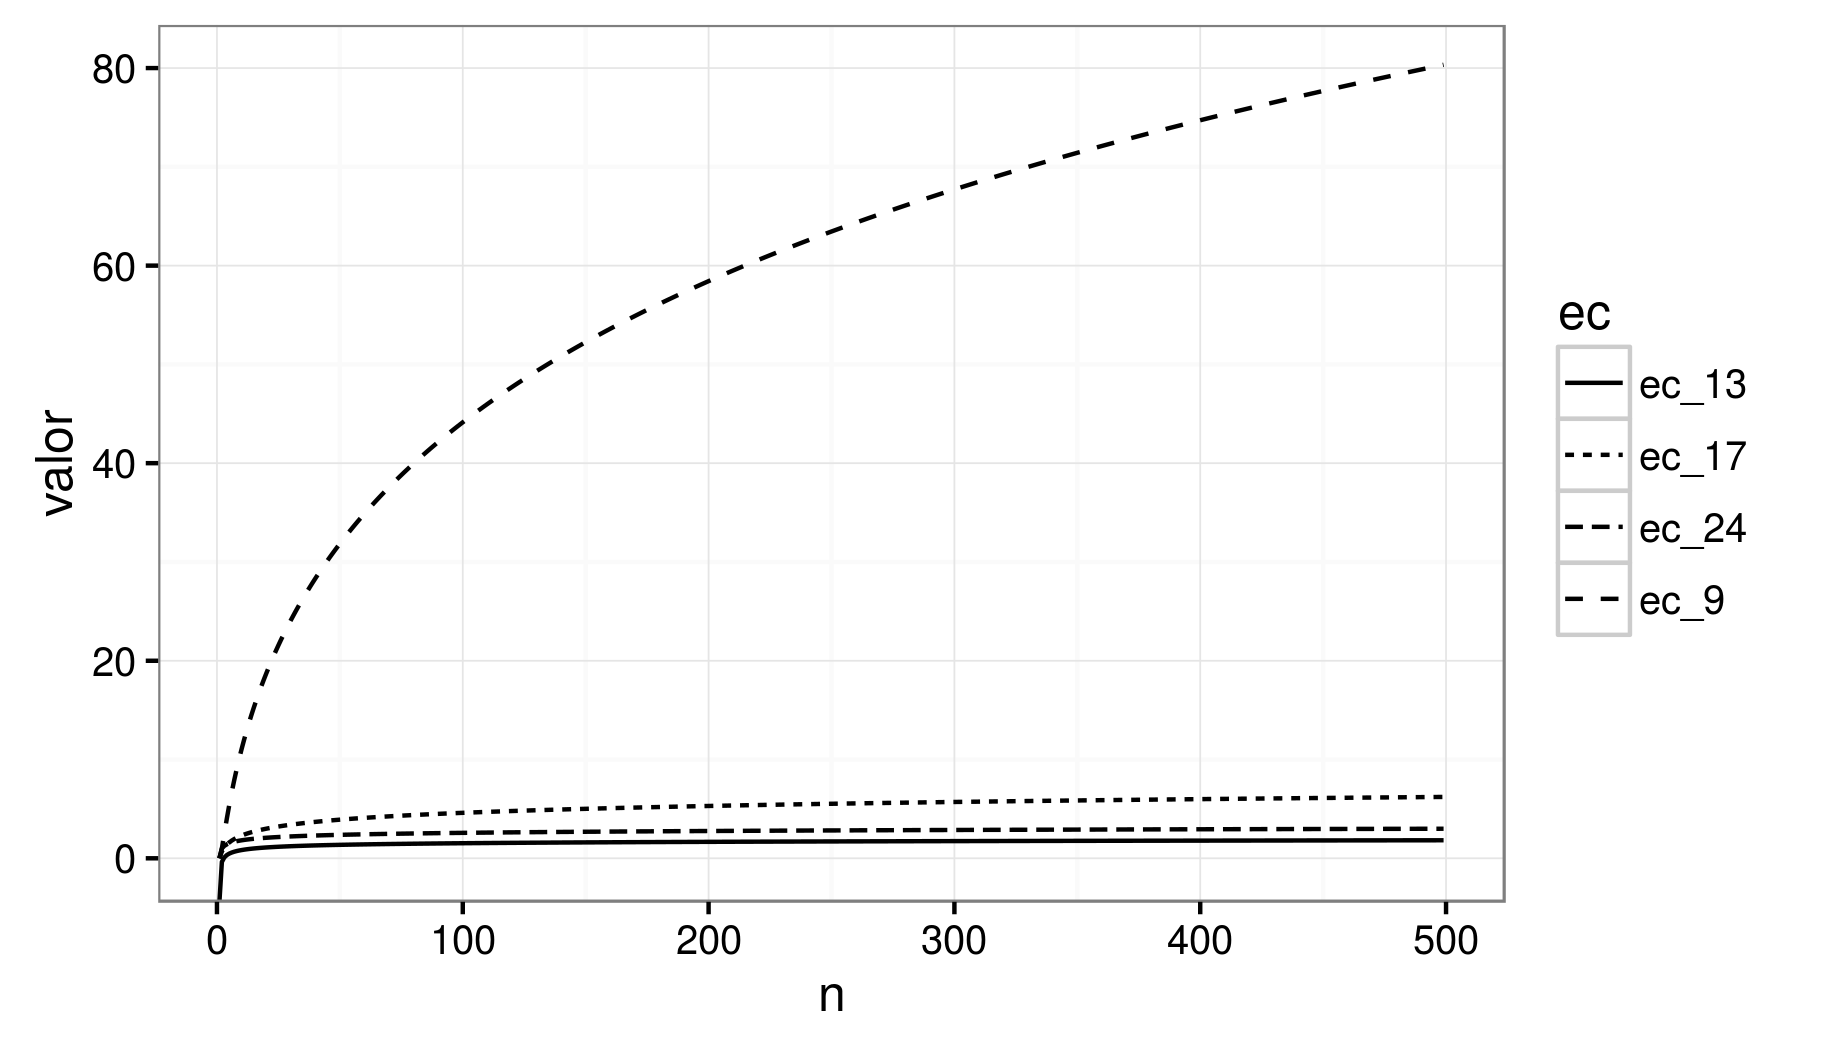
\includegraphics[width=0.5\textwidth]{img/graf_06.png}
\end{figure}

\begin{figure}[H]
\centering
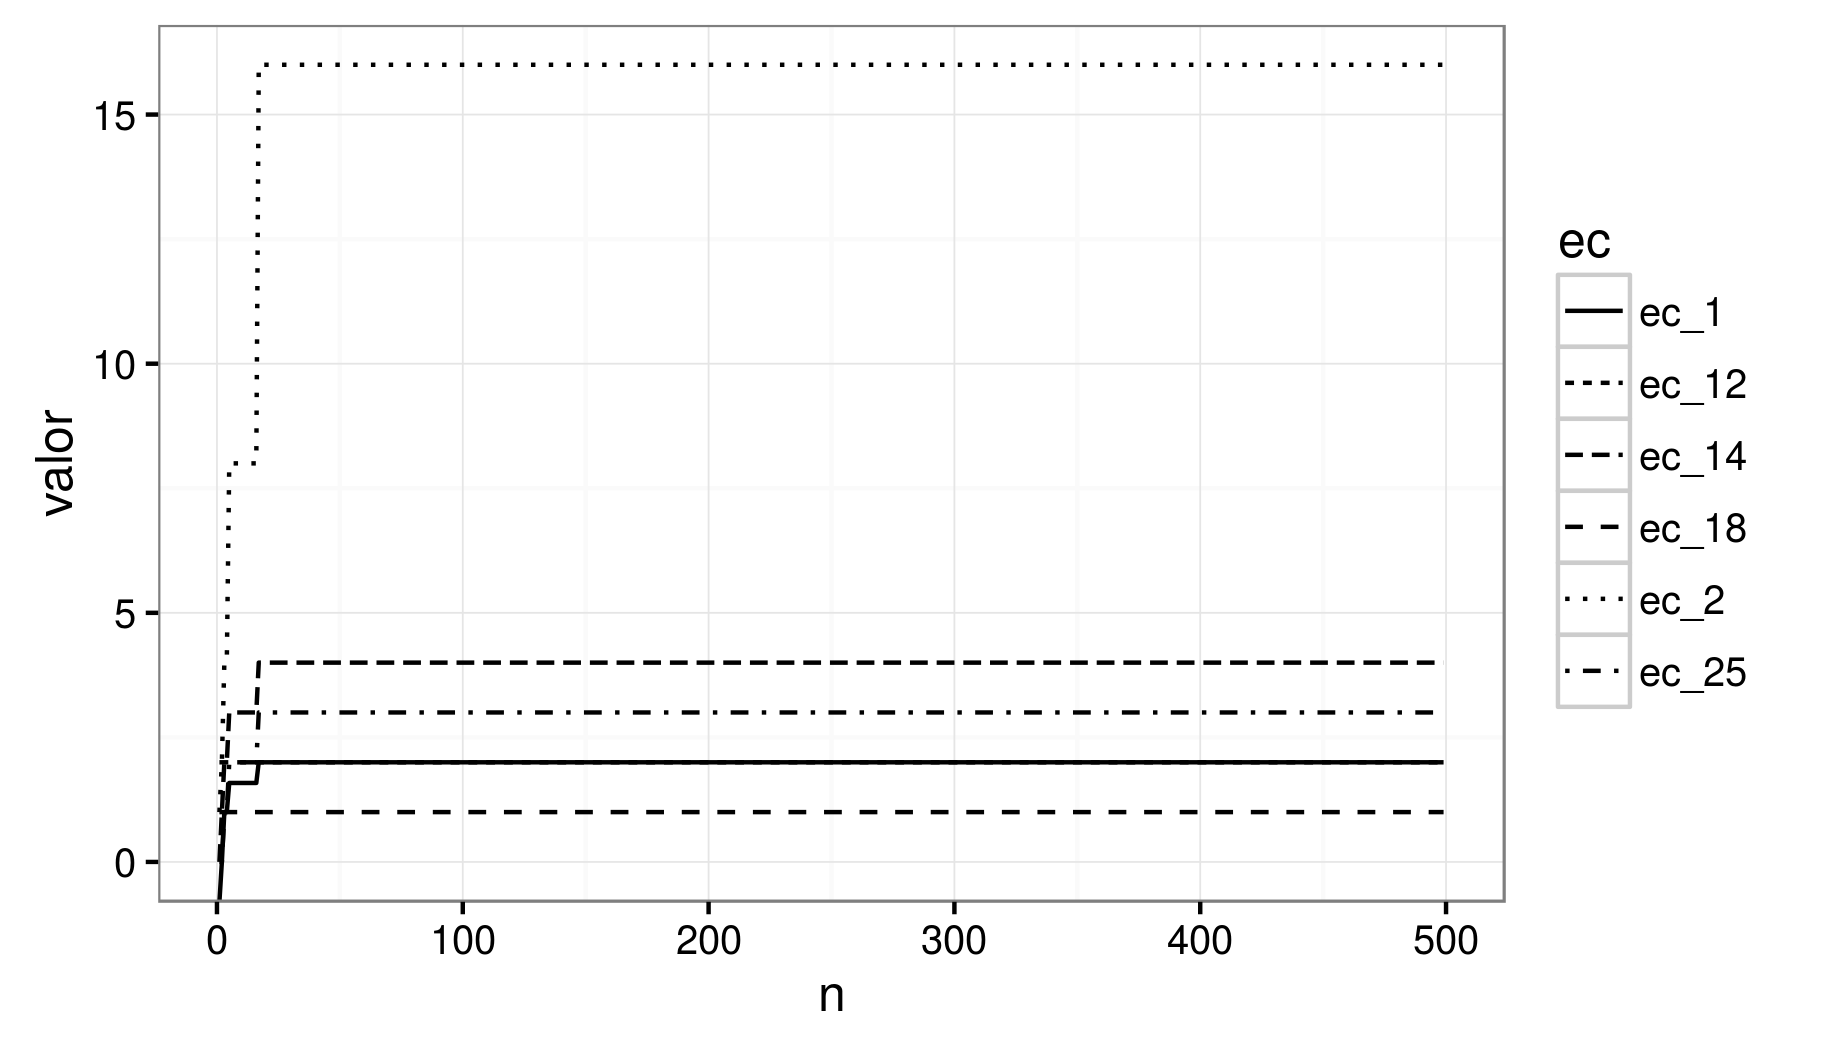
\includegraphics[width=0.5\textwidth]{img/graf_07.png}
\end{figure}

\end{document}
